\documentclass[11pt]{article}
\usepackage{amsmath,amssymb,amsthm}
\usepackage{graphicx}
\usepackage{geometry}
\usepackage{hyperref}
\geometry{margin=1in}

\title{A Precision-Controlled Null Result for a Khinchin-Signature PSLQ Family}
\author{Draft scaffold}
\date{April 2026}

\begin{document}
\maketitle

\begin{abstract}
We test whether simple low-dimensional integer relations occur among coordinates derived from the empirical Khinchin-signature statistic $S_n$, evaluated on the continued-fraction partial quotients of $\pi$. Using agreement across 256-, 512-, and 1024-bit runs, we isolate the maximal certified segment $n=1,\ldots,91$ and perform PSLQ searches on six fixed 3D/4D templates at 300-digit working precision with 600-digit confirmation. Under the conservative bound $\texttt{maxcoeff}=10^3$ and residual threshold $10^{-20}$, all $546$ template-specific attempts are unsupported. A wide-cap diagnostic rerun with $\texttt{maxcoeff}=10^6$ yields only high-coefficient fits, concentrated almost entirely in the 4-dimensional template, and these disappear completely when the conservative cap is restored. The outcome is therefore a reproducible, precision-controlled null result for the tested coordinate family rather than evidence of hidden arithmetic dependence.
\end{abstract}

\section{Numerical Experiments}\label{sec:numerics}

\subsection{Setup}
We worked with the stability-certified prefix $n=1,\ldots,91$ obtained by comparing the 256-, 512-, and 1024-bit runs and retaining the maximal contiguous range on which both $L_n$ and $S_n$ agreed to within $10^{-20}$ in absolute value. On this masked dataset we tested six fixed PSLQ templates drawn from the coordinate family $\{S_n,\, \log S_n,\, S_n-K_0,\, \log n\}$, using 300-digit working precision, 600-digit confirmation, residual threshold $10^{-20}$, confirmation threshold $10^{-10}$, and main coefficient cap $\texttt{maxcoeff}=10^3$.

\subsection{Results}
The conservative sweep comprised 546 template-specific attempts, distributed uniformly across the six templates. Every attempt was classified \emph{unsupported}, producing a clean null result for the tested coordinate family. The template definitions and wide-cap comparison counts are listed in Table~\ref{tab:templates}.

\input{agent_h_table1.tex}

\subsection{Diagnostic wide-cap comparison}
For comparison, we retained a previously saved diagnostic run with $\texttt{maxcoeff}=10^6$. Non-unsupported fits appeared only in T3 (1 hit) and T7 (90 hits), with T7 dominating the high-coefficient regime. Because these candidates vanish under the conservative cap, they are best interpreted as numerical artefacts rather than robust arithmetic structure.

\begin{figure}[t]
\centering
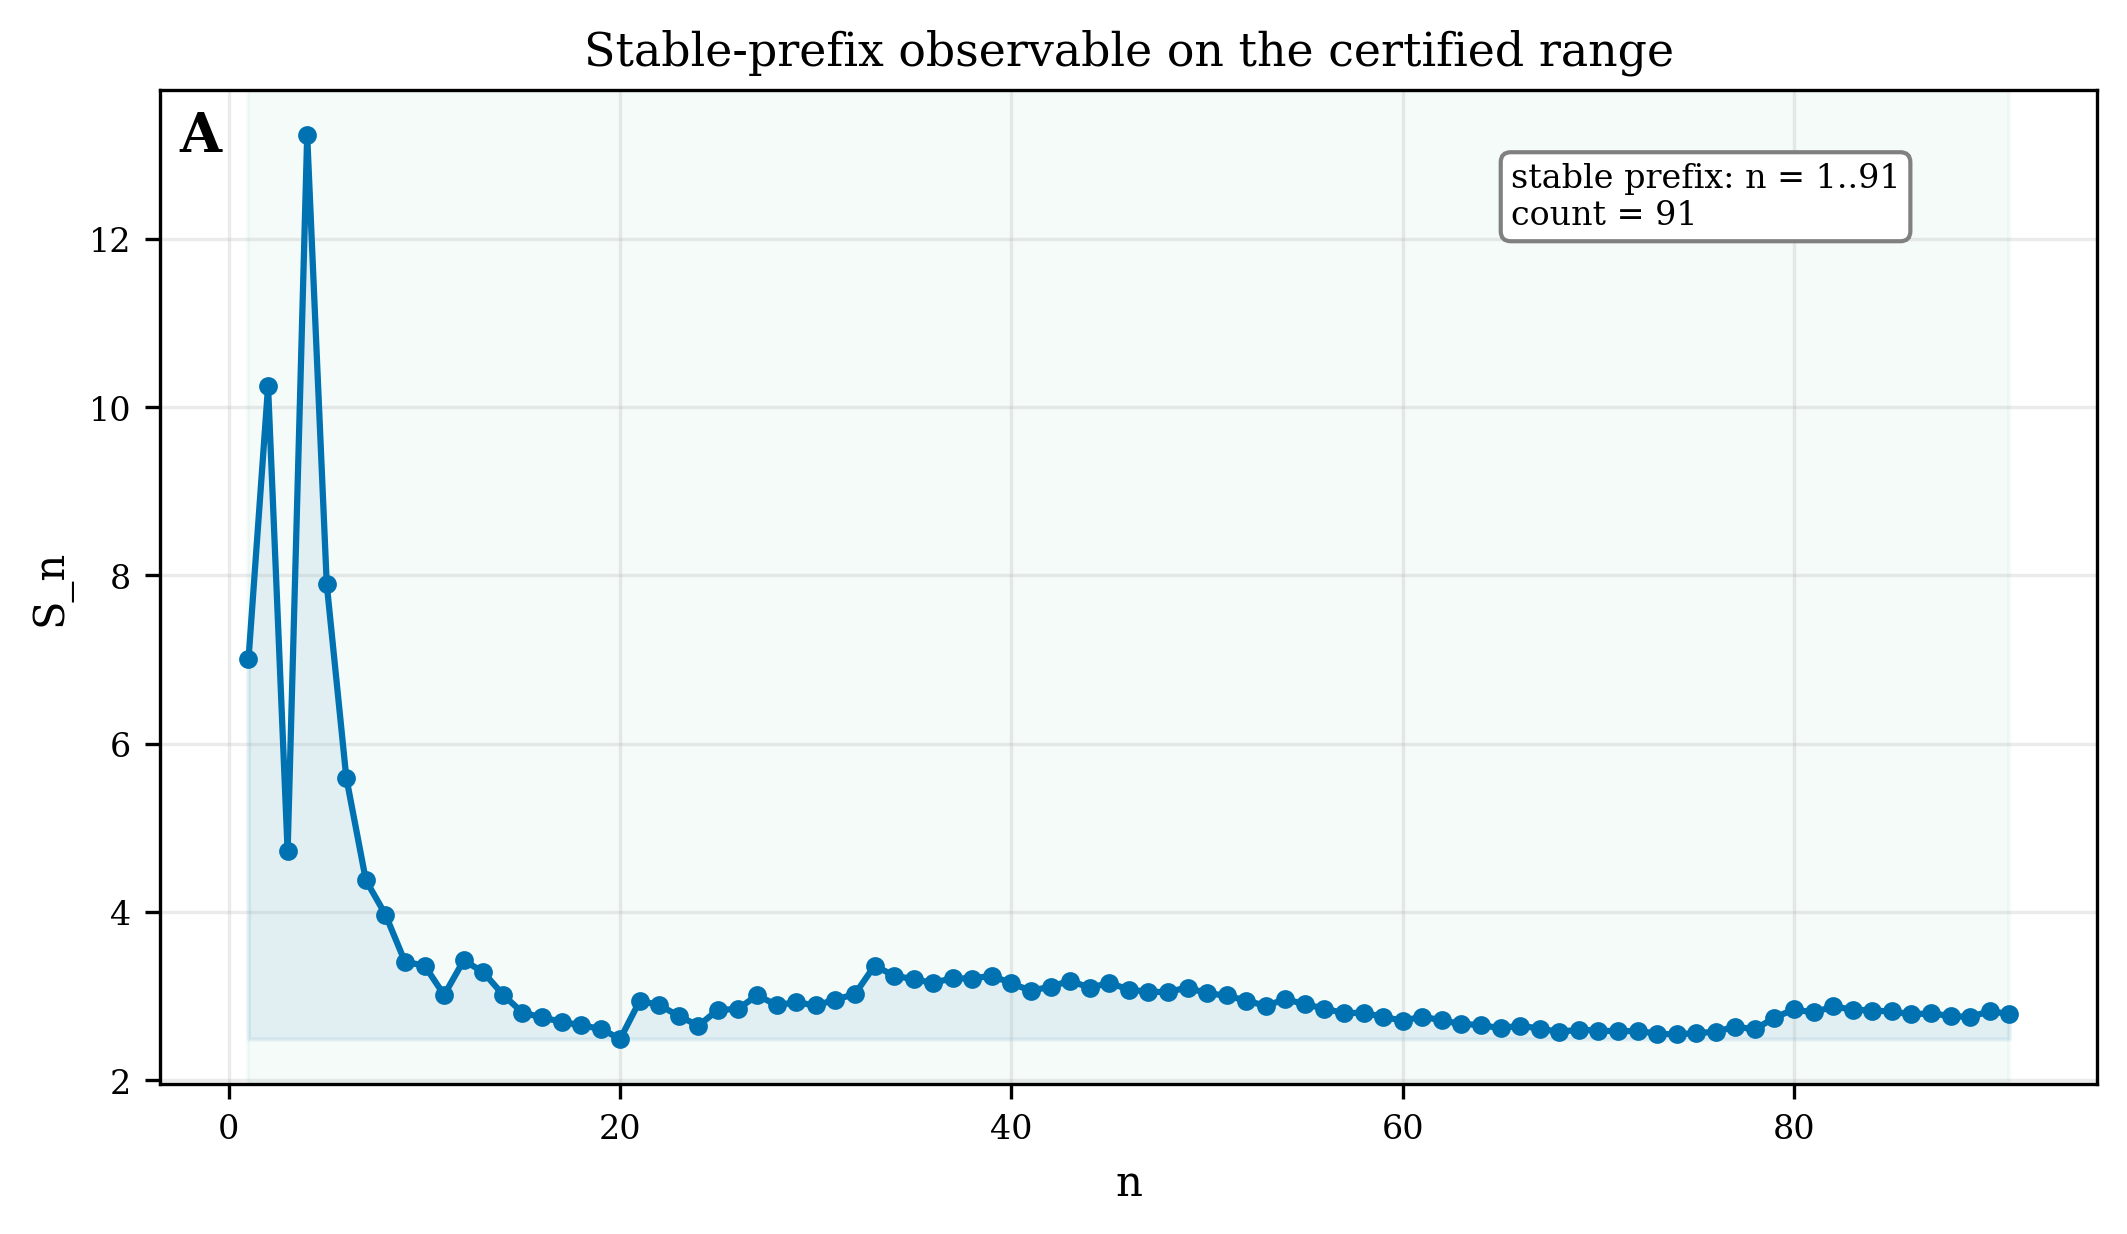
\includegraphics[width=0.48\linewidth]{figures/figure1_stable_prefix.png}\hfill
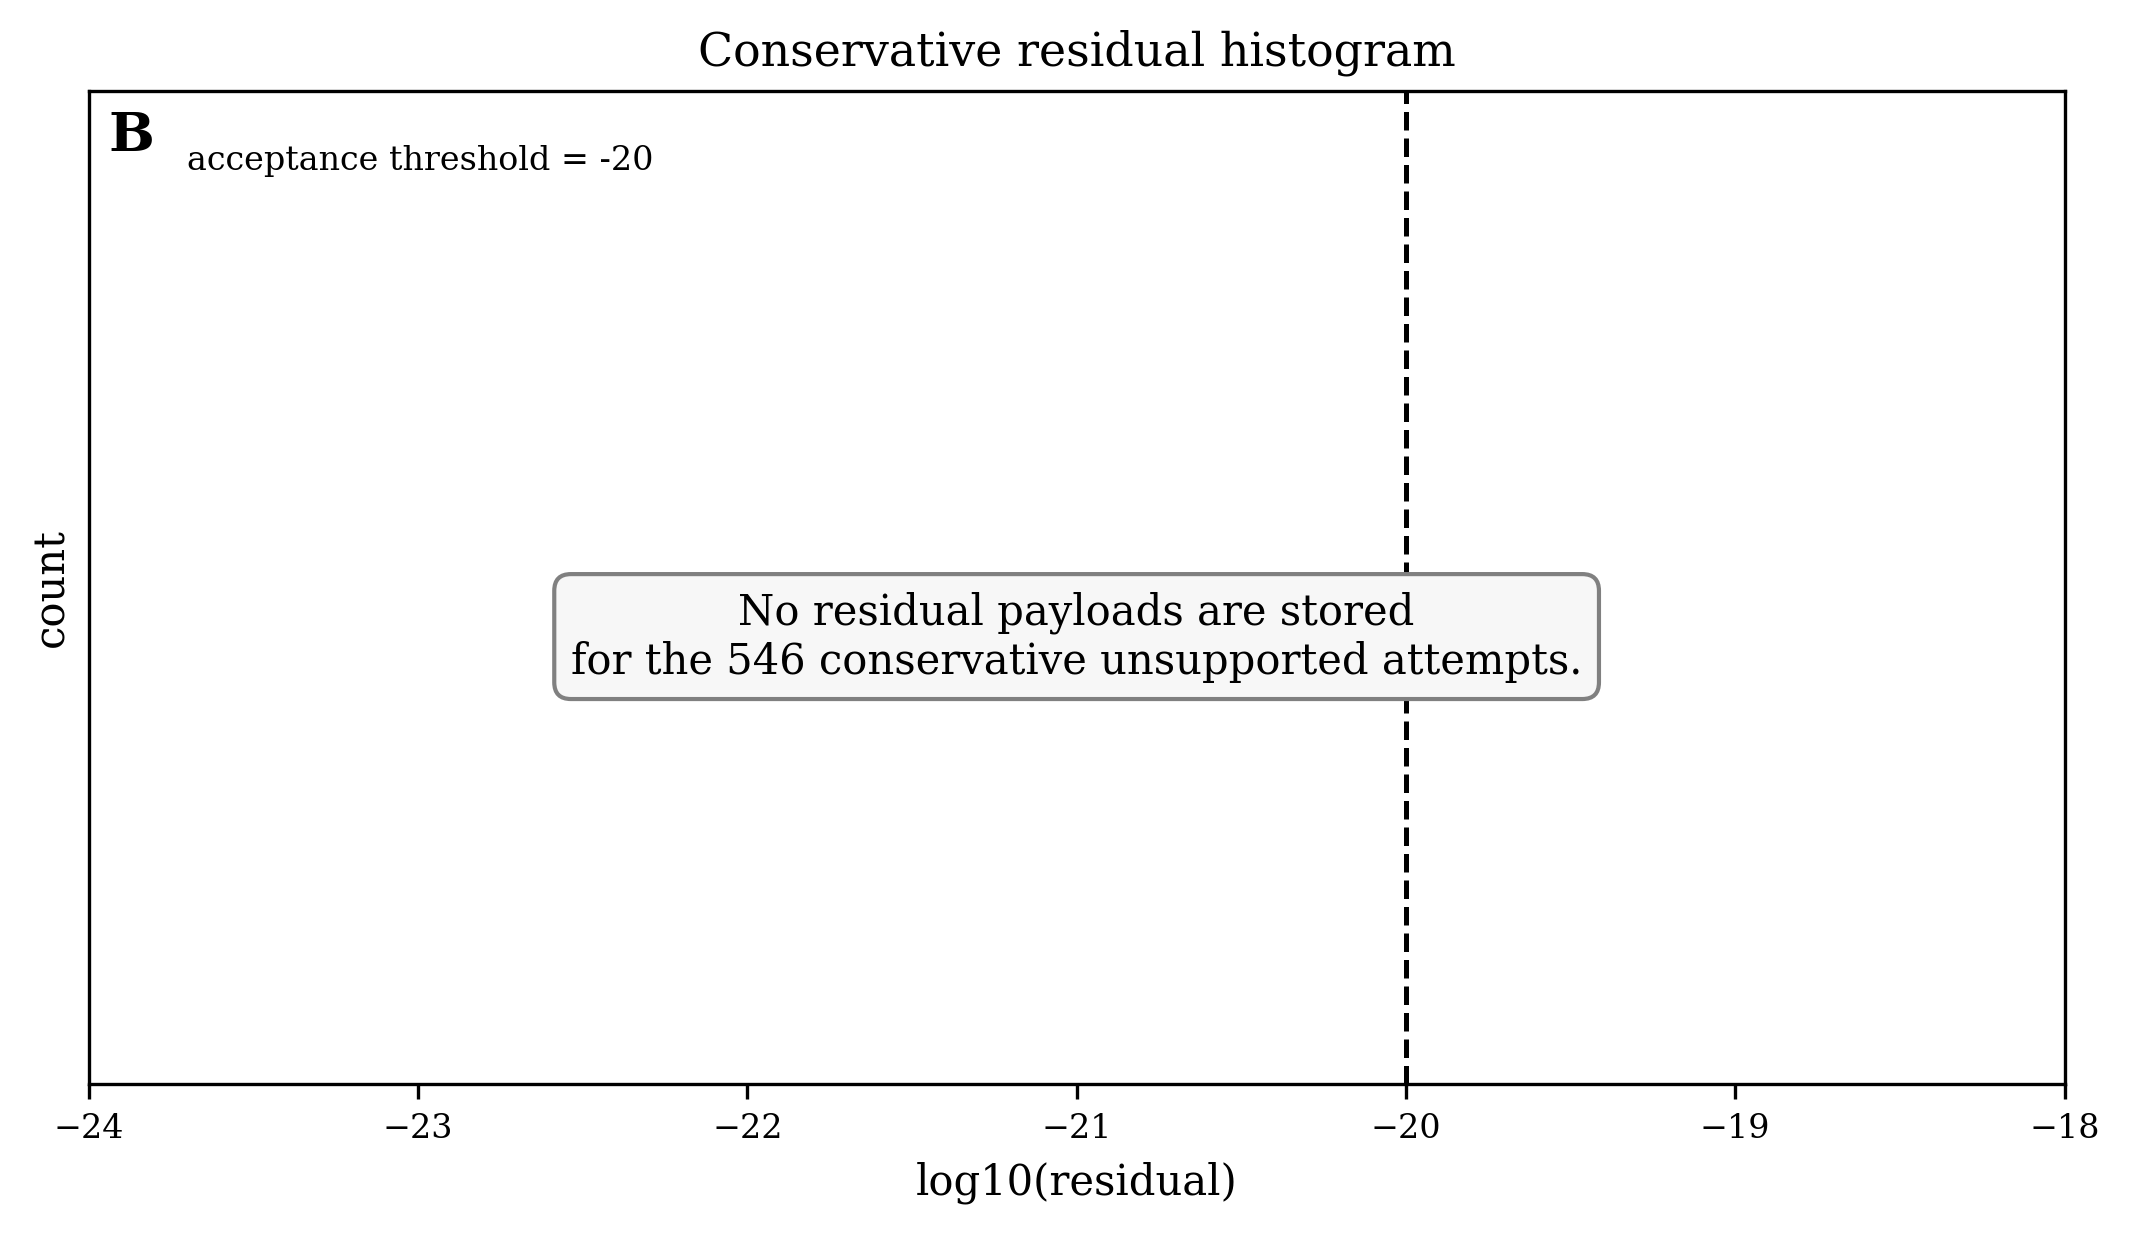
\includegraphics[width=0.48\linewidth]{figures/figure2_conservative_residual_hist.png}

\medskip

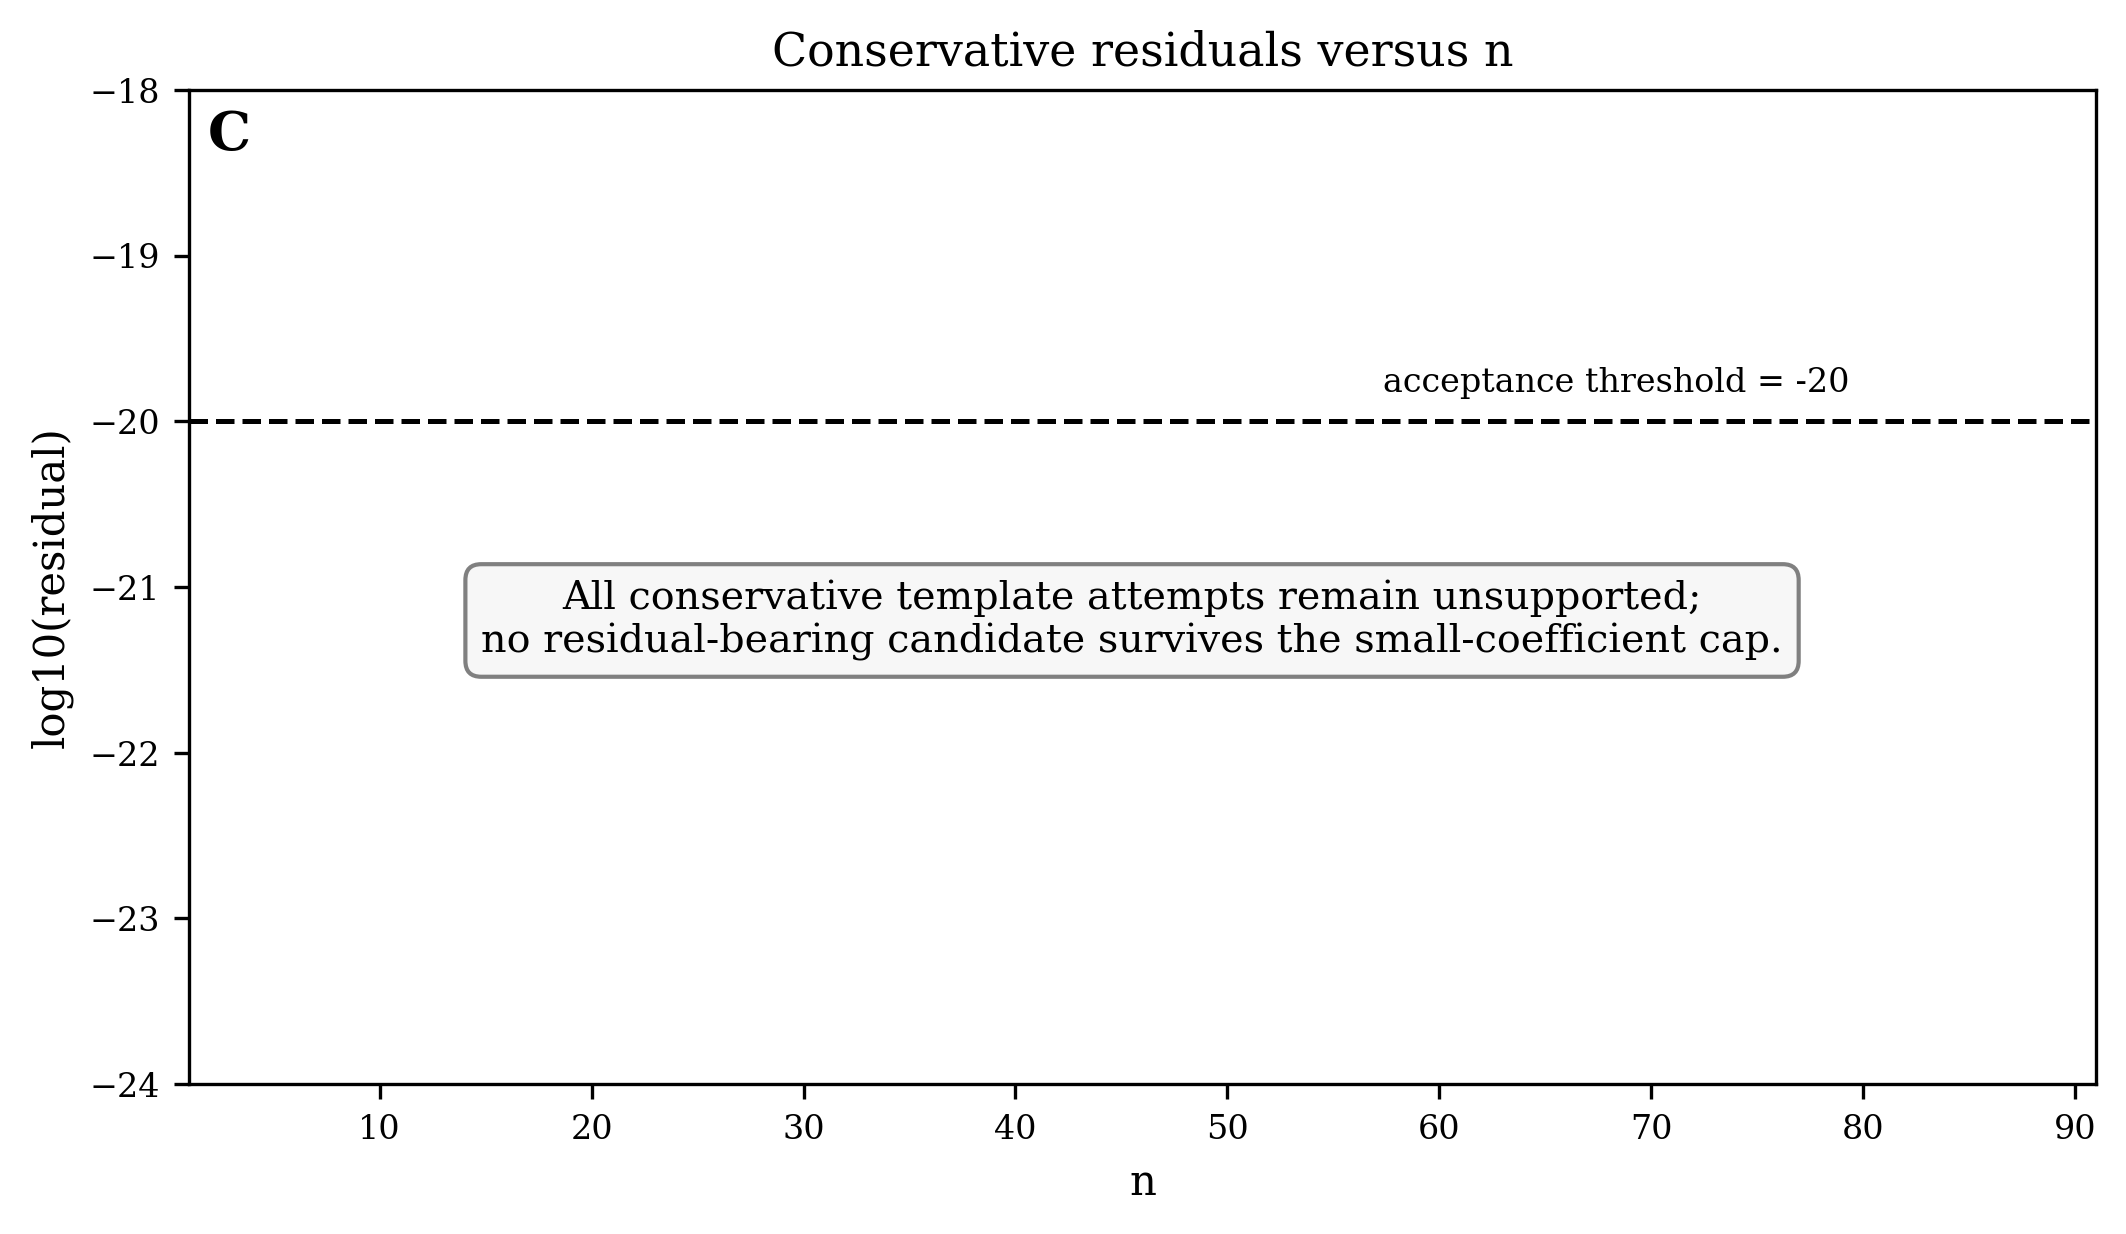
\includegraphics[width=0.48\linewidth]{figures/figure3_conservative_residuals_vs_n.png}\hfill
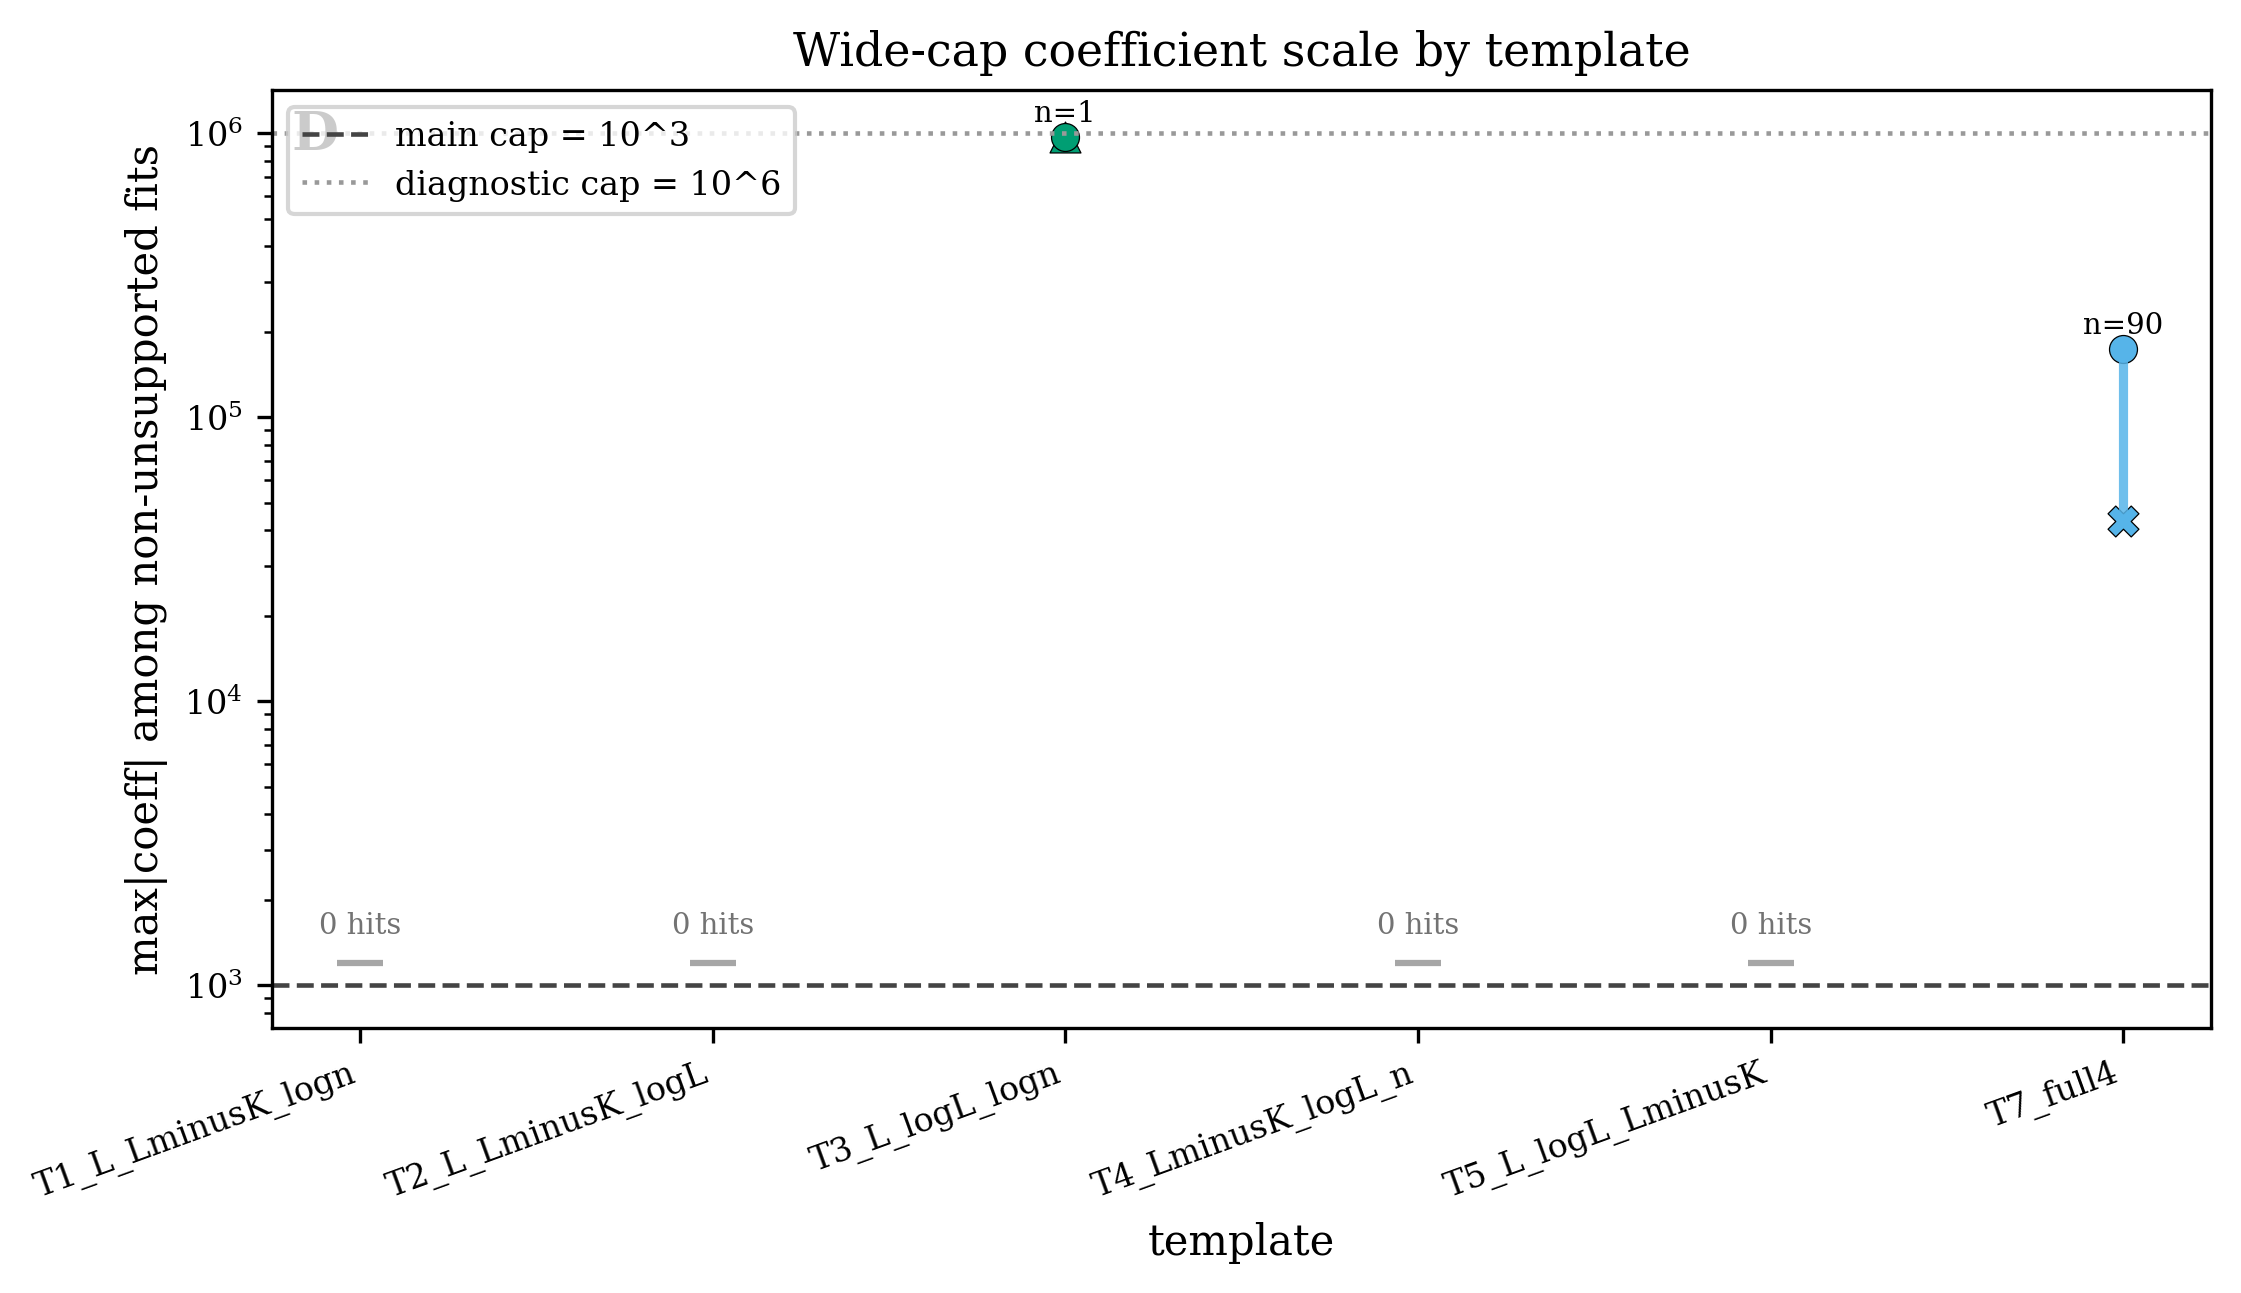
\includegraphics[width=0.48\linewidth]{figures/figure4_widecap_coeff_scale.png}
\caption{Masked Khinchin-signature PSLQ diagnostics. Upper left: the certified stable prefix. Upper right and lower left: conservative null-result panels with the $10^{-20}$ acceptance threshold. Lower right: coefficient scale for the wide-cap diagnostic fits, showing that the apparent hits are concentrated in large-coefficient regimes.}
\label{fig:khinchin_panels}
\end{figure}


\section{Discussion}

The numerical evidence supports a disciplined negative conclusion: within the tested coordinate family $\{S_n,\, \log S_n,\, S_n-K_0,\, \log n\}$, no low-complexity integer relation survives simultaneous precision filtering, stability masking, and a conservative small-coefficient PSLQ search. This is informative because it separates genuine structural absence from the high-coefficient artefacts that arise when the search volume is enlarged dramatically.

At the same time, the null result is deliberately local in scope. It does not rule out relations involving richer nonlinear functions of the index, alternative normalizations, or coordinate families augmented by additional constants or transforms. For instance, templates involving $n^{1/2}$, $n^2$, or algebraic combinations of $K_0$ with other known constants lie entirely outside the tested family and remain open. Nor does it exclude the possibility that qualitatively new behaviour could emerge beyond the presently certified prefix if higher-precision stabilization makes a longer trusted window available.

For referee credibility, this distinction is essential: the present work certifies the absence of simple relations in a concrete, reproducible regime, rather than claiming a universal impossibility theorem. The natural next steps are to repeat the masked workflow on other well-studied constants, to enlarge the coordinate library in a controlled way, and to compare the observed null regime with symbolic models that predict when PSLQ should and should not succeed. High-quality null results of this kind are an essential calibration for any future positive claim of arithmetic structure in continued-fraction data.

\section*{Computational and AI Disclosure}

The computational experiments, precision-controlled PSLQ searches, stability masking, and diagnostic analyses in this paper were conducted within a multi-agent research workflow combining GitHub Copilot (in Visual Studio Code) for code generation, iterative refinement, and workspace-level automation, and Anthropic Claude for strategic guidance, mathematical review, and synthesis across project stages. All numerical results, proofs, and mathematical claims were independently verified by the author using reproducible Python scripts and archived artifacts. The full codebase, residual logs, status-block JSON files, and figure sources supporting this work are publicly available at \url{<INSERT_GITHUB_URL_HERE>}.


\begin{thebibliography}{9}
\bibitem{AEAL2025} Papanokechi, \emph{AEAL: Agent Epistemic Accountability Layer --- A Framework for Verifiable AI-Assisted Research}, Zenodo (2025), doi:10.5281/zenodo.19562751.
\end{thebibliography}

\end{document}
